\paragraph{QuizziPedia::Front-End::ModelViews::FillingQuestionsModelView}
\begin{figure} [ht]
	\centering
	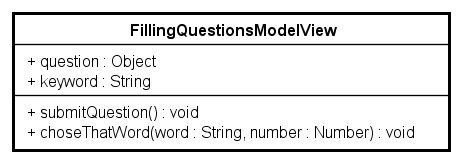
\includegraphics[scale=0.80]{UML/Classi/Front-End/QuizziPedia_Front-end_ModelView_FillingQuestionsModelView.png}
	\caption{QuizziPedia::Front-End::ModelViews::FillingQuestionsModelView}
\end{figure} \FloatBarrier
\begin{itemize}
	\item \textbf{Descrizione}: classe di tipo modelview la cui istanziazione è contenuta all'interno della variabile di ambiente \texttt{\$scope} di \textit{Angular\ped{G}}. All'interno di essa sono presenti le variabili e i metodi necessari per il \textit{Two-Way Data-Binding\ped{G}} tra la \textit{view\ped{G}} \texttt{FillingQuestionsView} e il \textit{controller\ped{G}} \texttt{FillingQuestionsController}; 
	\item \textbf{Utilizzo}: viene utilizzata per effettuare il \textit{Two-Way Data-Binding\ped{G}} tra la \textit{view\ped{G}}\\ \texttt{FillingQuestionsView} e il \textit{controller\ped{G}} \texttt{FillingQuestionsController} rendendo disponibili variabili e metodi;
	\item \textbf{Relazioni con altre classi}:
	\begin{itemize}
		\item \textbf{IN \texttt{FillingQuestionsView}}: \textit{view\ped{G}} contenente i campi e le direttive per creare una domanda a riempimento testo; 
		\item \textbf{IN \texttt{FillingQuestionsController}}: questa classe permette di gestire la creazione e la modifica di una domanda a riempimento di spazi.
	\end{itemize}
	\item \textbf{Attributi}:
	\begin{itemize}
		\item \texttt{+ question: Object} \\ Oggetto contenente gli attributi per la creazione della domanda:
		\begin{itemize}
			\item \texttt{answer: Array}: \texttt{array} contenente oggetti che rappresentano le risposte. Ogni oggetto risposta contiene:
			\begin{enumerate}
				\item \texttt{wordNumber: Number}: attributo di tipo \texttt{Number} che indica la parola nel testo che andrà inserita in fase di compilazione.
			\end{enumerate}
		\end{itemize}
		\item \texttt{+ keyword: String} \\ Attributo contenente la keyword associata alla domanda/questionario.
	\end{itemize}
	\item \textbf{Metodi}:
	\begin{itemize}
			\item \texttt{+ submitQuestion(): void}\\ 
			Metodo che gestisce l’evento click sul pulsante di conferma sulla domanda. Raccoglie i dati dal modelview e li manda al server attraverso \texttt{QuestionService}. Poi verrà effettuato il redirect alla pagina di gestione delle domande oppure al questionario che si stava creando; 
			\item \texttt{+ choseThatWord(word: String, number: Number): void}\\
			Metodo che gestisce l’evento click su una parola del testo. Una volta selezionata essa verrà inserita nell'array che conterrà le parole che dovranno essere nascoste quando l'esercizio sarà proposto. \\
			\textbf{Parametri}:
			\begin{itemize}
				\item \texttt{word: String} \\
				Parametro contenente la parola scelta da nascondere;
				\item \texttt{number: Number} \\ 
				Parametro che si riferisce al numero della parola scelta da nascondere.
			\end{itemize}
	\end{itemize}
\end{itemize}

